\documentclass[]{article}

\usepackage[utf8]{inputenc}

\usepackage[T1]{fontenc}

\usepackage[english]{babel}

\usepackage{amsmath, amsfonts, amssymb, amsthm}

\usepackage{fullpage}

\usepackage{enumerate}
\usepackage{graphicx}
\usepackage{algorithm}
\usepackage{algorithmic}

\usepackage{hyperref}
\hypersetup{
    colorlinks,
    citecolor=black,
    filecolor=black,
    linkcolor=black,
    urlcolor=black
}


%Pour les algos
\floatname{algorithm}{Algorithme}
\renewcommand{\algorithmicrequire}{\textbf{Entrée:}}
\renewcommand{\algorithmicensure}{\textbf{Sortie:}}
\renewcommand{\algorithmicif}{\textbf{si}}
\renewcommand{\algorithmicthen}{\textbf{alors}}
\renewcommand{\algorithmicelse}{\textbf{sinon}}

\title{
{\Huge Speaker classification project}\\
Signal processing\\
}

\author{
\textbf{Dell’Aria Doriano}
\and
\textbf{Goffaux Lionel}\\
}

\date{\today\\
Academic Year 2020-2021\\
Bachelor's degree in Computer Science\\}

\begin{document}

\maketitle
\pagebreak

% \tableofcontents
% \pagebreak

\section{Introduction}
In this project, we are going to extract features of a set of voice samples, to be able to classify if the sample is a
male or female voice.

\section{Energy}
In the \autoref{energy}, we plot the sample and its energy. We observe that with a threshold of 5,
we are able to classify the voiced and unvoiced frames.
Then we use these voiced frames to extract all the features we need.


\begin{figure}[H]
    \centering
    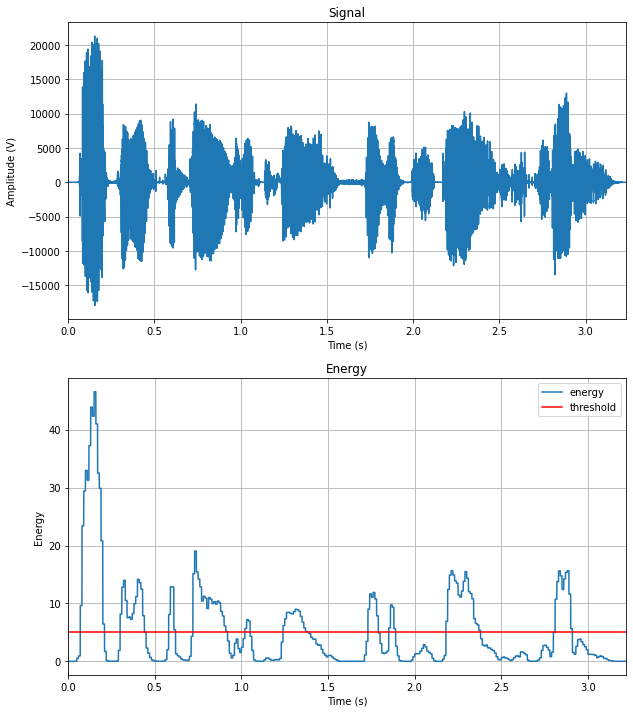
\includegraphics[scale=0.5]{images/energy_threshold.png}
    \caption{\label{energy}Energy of a sample}
\end{figure}

\section{Features extraction}
\subsection{Pitch}
They are multiple ways to extract the pitch of a sample. In our case, we extract the pitch with an autocorrelation-based
system and a cepstrum-based system.

\subsubsection{autocorrelation}
The principle of autocorrelation is to correlate the signal with itself. We first split the signal into frames then autocorrelate
frames with themselves.
So we obtain the pitch by measuring the distance between the distance of two peaks of the autocorrelation. 
we fix the frames width = 21, the step = 5 and the threshold = 5. 
In \autoref{autocorr}, we observe that the method doesn't have 100\% accuracy because we obtain pitch over 5000 Hz.

\begin{figure}[h]
    \centering
    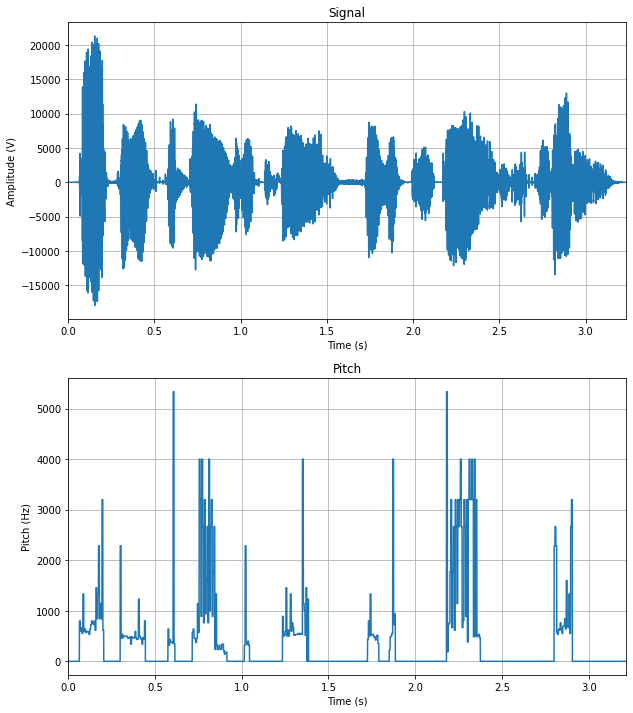
\includegraphics[scale=0.5]{images/autocorr_pitch.png}
    \caption{\label{autocorr}autocorrelation-based system}
\end{figure}

\subsubsection{Cepstrum}

\begin{figure}[H]
    \centering
    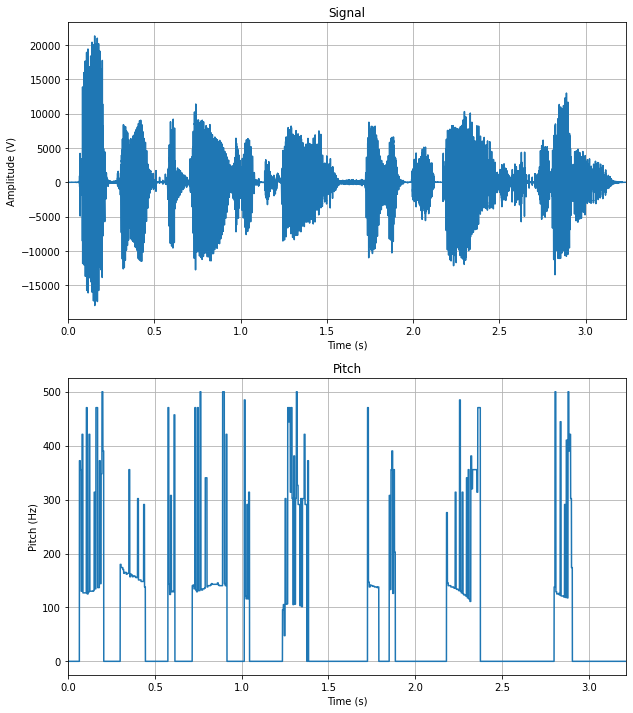
\includegraphics[scale=0.5]{images/cepstrum_pitch.png}
    \caption{\label{cepstrum}cepstrum-based system}
\end{figure}

\subsection{Formants}


\subsection{MFCC}

\section{Features visualization}

In order to determine on which features our rule-based system will rely upon, we will draw a
distribution graph of each sentence's feature, separating the two speakers. To do so, we will separate all
the features in three classes, the different pitch estimations, the formants and
the Mel-frequency cepstrum coefficients (MFCC). These observations will be made on sample of
15 sentences for each speaker.

\subsection{The pitch estimations}

For the pitch estimations, we have the two methods describe above. So for each sentence 
we take the mean's pitch of all the frames. We have also seen before that these estimations are
not always accurate and occasionally give us some outliers. Given that, we decide to calculate
the median value too which will be less sensitive to those.


\begin{figure}[H]
    \centering
    \caption{Pitch features}
    \label{pitch_visu}
    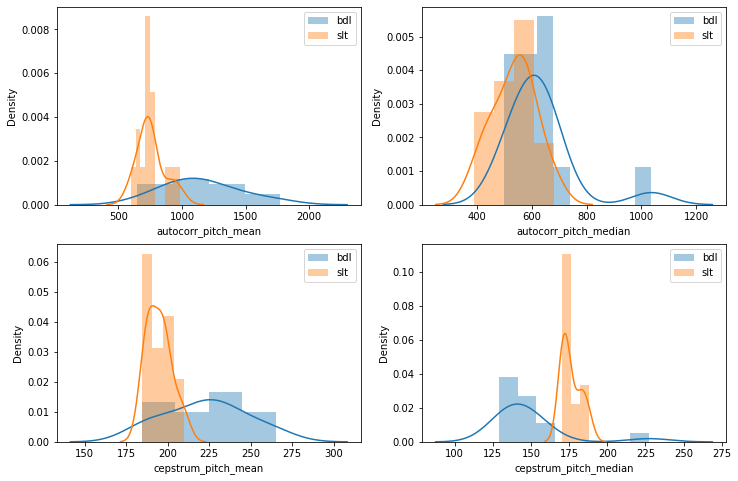
\includegraphics[scale=0.5]{images/pitch_visu.png} 
\end{figure}


On \autoref{pitch_visu}, we observe a good distinction between the speakers for the mean autocorrelation
and cepstrum pitch. We also see that the median value of the cepstrum pitch give us a good
discriminating feature.

\subsection{The Formants}


\begin{figure}[H]
    \centering
    \caption{\label{formants_visu}Formants features}
    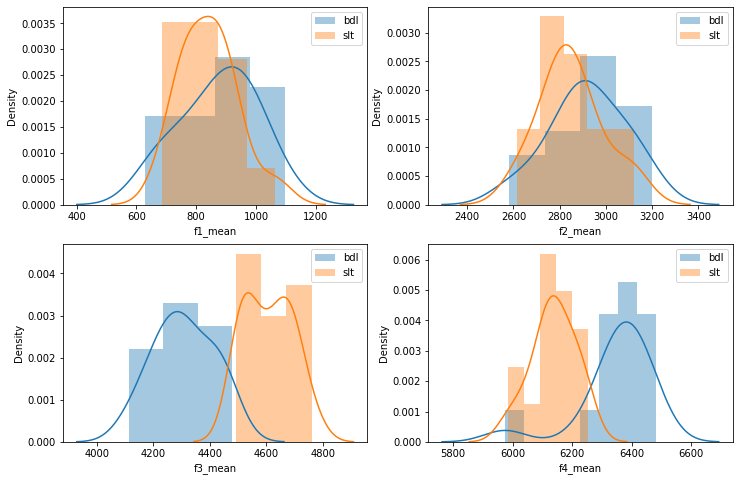
\includegraphics[scale=0.5]{images/formants_visu.png}
\end{figure}

For the formants we use the same methode as before by calculating the mean of the frames for
each formant. We can see on \autoref{formants_visu} that more interesting formants are the two
last ones. For the formants 1 and 2, they look almost similar for the two speakers.

\subsection{The MFCC}

In the same way, we take for each MFCC the mean of each sentence's frames. Considering
the number of MFCC, we have only taken the most relevant ones on \autoref{mfcc_visu}. 

\begin{figure}[H]
    \centering
    \caption{\label{mfcc_visu}The most interesting MFCC features}
    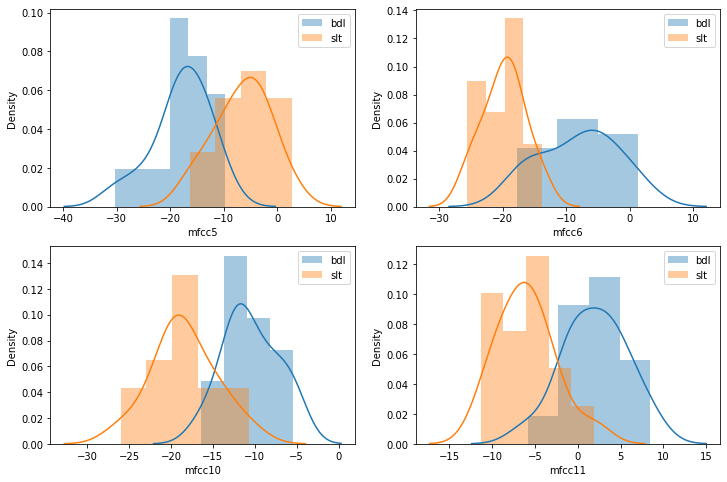
\includegraphics[scale=0.5]{images/mfcc_visu.png}
    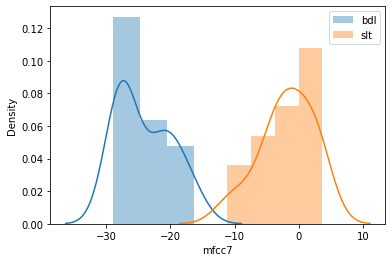
\includegraphics[scale=0.5]{images/mfcc7_visu.png}
\end{figure}

As we can see, the seventh MFCC is a perfect discriminant of two speakers. In fact,
if we observe a larger sample of sentence we find that there is bit of overlapping 
between the two but this feature stays from far the most convenient to make the
speaker classification.

\section{Rule-Based system}

In this section, we will use what we have learned from the features observation we have 
done previously to build simple rule-based system which will determine which speaker is
speaking. Each system will be test on 50 random sentences for each speaker.

\subsection{The MFCC system}

A first approach is to use the MFCC 7 feature and define a threshold to separate the two speakers.
After some tries, we have found that $-12$ dB is a good limit. After implementation, we get a model
with $100\%$ accuracy.


\begin{figure}[H]
    \centering
    \caption{\label{confusion1}MFCC confusion matrix}
    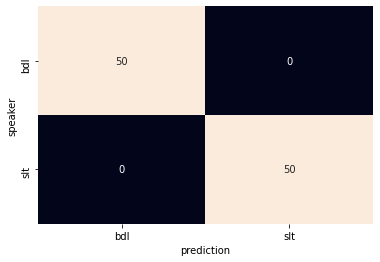
\includegraphics[scale=0.5]{images/confusion1.png}
\end{figure}

\subsection{The median cepstrum pitch system}

For this second model we use the median cepstrum pitch estimation to make the classification.
If the sentence have a pitch between 165 and 200 Hz we consider it as a  slt's one.
With this model we have $99\%$ accuracy.

\begin{figure}[H]
    \centering
    \caption{\label{confusion2}Median cepstrum pitch confusion matrix}
    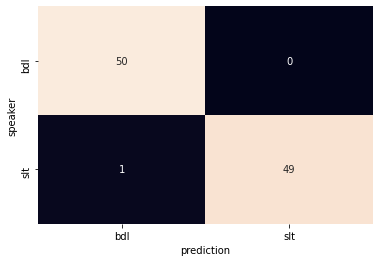
\includegraphics[scale=0.5]{images/confusion2.png}
\end{figure}

\subsection{The third formant system}

\begin{figure}[H]
    \centering
    \caption{\label{confusion3}Third formant confusion matrix}
    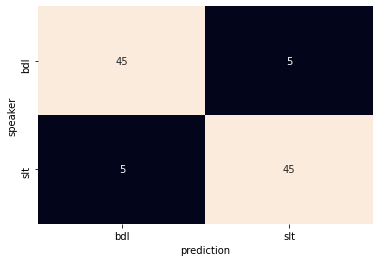
\includegraphics[scale=0.5]{images/confusion3.png}
\end{figure}

This model is based on the third formant feature. If this feature has a frequency above 4470 Hz, 
we consider that the sentence is from slt. With this one we get $96\%$ accuracy.

\section{Machine learning}

Now, we will see if we can do the same using machine learning. We will try a first model and then
try to improve is performance. For these we need to take a bigger sample in order to have a test set
with more or less 100 sample like the previous section and also a train set to train the model.

\subsection{Decision tree classifier}

First, we will try a simple decision tree classifier. This will more or less like we did manually before
but it will explore mush more possibilities to get the highest score. With this model we get 98\% accuracy.
We can visualize on autoref{learncurve1} the learning curve of our model.


\begin{figure}[H]
    \centering
    \caption{\label{learncurve1}Decision tree's learning curve}
    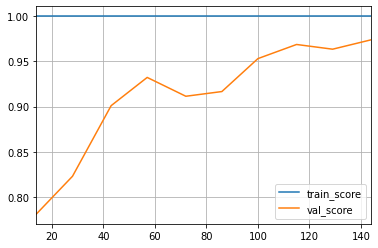
\includegraphics[scale=0.5]{images/learncurve1.png}
\end{figure}

\subsection{Random forest}

In order to reach the 100\% accuracy, we will use a random forest classifier. This model
generates randomly several trees and then take the average of their result. The idea beyond
that is that if some of them make a mistake the orders will have the good result because they
are all slightly different. We can visualize on \autoref{learncurve2} that this one reach 
well 100\% accuracy.


\begin{figure}[H]
    \centering
    \caption{\label{learncurve2}Random forest's learning curve}
    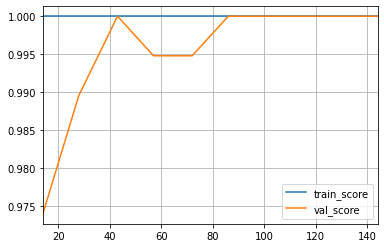
\includegraphics[scale=0.5]{images/learncurve2.png}
\end{figure}

Another solution to improve our first tree is to just keep the most important features and
delete the others. We could do a statistical test to determine those features.

\section{Conclusion}


With all we know now, we can answer the main question of this project.
What are the advantages of machine learning-based systems? Here, with
a simple rule-based system, we got a result as good as the machine learning's one. 
But it's due to fact that we had a good dataset with a good features extraction.
We had some features which are basically a direct indicator of the target. In more
complicated cases, the features we need to use isn't so clear. It's hard to say which one
is the most important and how can use it with the others to have the higher accuracy possible.
The advantage of machine learning is that we let that to the machine. For this project, for instance,
we can see on \autoref{feat_imp} the importance of each feature according to the random forest we created.

\begin{figure}[H]
    \centering
    \caption{\label{feat_imp}Feature importance}
    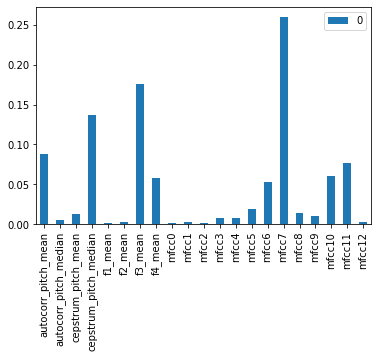
\includegraphics[scale=0.7]{images/feat_imp.png}
\end{figure}

% ====== exemple d'algo =======
% \begin{algorithm}
%     \caption{Recherche linéaire du maximum}
%     \begin{algorithmic}[1]
%     \REQUIRE un tableau d’entiers $A$
%     \ENSURE la valeur du plus grand entier contenu dans $A$
%     \STATE $max \leftarrow -\infty$
%     \FOR{$i \leftarrow 1$ `a $longueur[A]$}
%     \IF{$max < A[i]$}
%     \STATE $max \leftarrow A[i]$
%     \ENDIF
%     \ENDFOR
%     \RETURN $max$
%     \end{algorithmic}
% \end{algorithm}


\end{document}